\documentclass[10pt,a4paper]{article}
\usepackage[a4paper,margin=18mm,headheight=15pt]{geometry}
\usepackage{fontspec}
\usepackage{microtype}
\usepackage{xcolor}
\usepackage{booktabs}
\usepackage{tabularx}
\usepackage{array}
\usepackage{enumitem}
\usepackage{fancyhdr}
\usepackage{hyperref}
\usepackage[most]{tcolorbox}
\usepackage{listings}
\usepackage{tikz}
\usetikzlibrary{positioning,arrows.meta}
% Generated from certificate.json. Do not edit by hand.
\newcommand{\AreaHigh}{15.6531}
\newcommand{\AreaImprovement}{15.5943}
\newcommand{\AreaLosses}{0}
\newcommand{\AreaLow}{15.5355}
\newcommand{\AreaWins}{64}
\newcommand{\BaselineArea}{33,892,339}
\newcommand{\BaselineDelay}{11.1642}
\newcommand{\BaselineFmax}{89.5717}
\newcommand{\BaselineHash}{c2472728e2d52b29ad451f5c9779ebb749c318e9be048d03e6a6555c735eda53}
\newcommand{\BaselinePower}{22.4567}
\newcommand{\CertificateHash}{e77ed39c79559af8cbbd2efeaf4fb67045740684ac4fc35699213c3cc1858906}
\newcommand{\CertificationPairs}{64}
\newcommand{\CompositeHigh}{8.4462}
\newcommand{\CompositeImprovement}{8.3230}
\newcommand{\CompositeLosses}{0}
\newcommand{\CompositeLow}{8.1997}
\newcommand{\CompositeWins}{64}
\newcommand{\DelayHigh}{3.7855}
\newcommand{\DelayImprovement}{3.1868}
\newcommand{\DelayLosses}{10}
\newcommand{\DelayLow}{2.5843}
\newcommand{\DelayWins}{54}
\newcommand{\FunctionalTests}{151}
\newcommand{\OptimizedArea}{28,607,064}
\newcommand{\OptimizedDelay}{10.8085}
\newcommand{\OptimizedFmax}{92.5202}
\newcommand{\OptimizedHash}{25327189f78f238e909fa5940afff9e2b000547336cdc614ee9ea9c4633aa11f}
\newcommand{\OptimizedPower}{21.1749}
\newcommand{\OptimizedScore}{0.916770}
\newcommand{\PowerHigh}{6.2509}
\newcommand{\PowerImprovement}{5.7081}
\newcommand{\PowerLosses}{0}
\newcommand{\PowerLow}{5.1622}
\newcommand{\PowerWins}{64}
\newcommand{\SearchPairs}{5}


\definecolor{Ink}{HTML}{15171A}
\definecolor{Blue}{HTML}{0878FF}
\definecolor{Pale}{HTML}{F1F5F9}
\definecolor{Muted}{HTML}{667085}
\definecolor{Green}{HTML}{087A55}
\hypersetup{colorlinks=true,linkcolor=Blue,urlcolor=Blue,pdftitle={INT8 MatVec RTL optimization - verified VTR45 evidence},pdfauthor={Göther Labs}}
\setmainfont{Helvetica Neue}
\setsansfont{Helvetica Neue}
\setmonofont{Menlo}
\renewcommand{\familydefault}{\sfdefault}
\setlength{\parindent}{0pt}
\setlength{\parskip}{5pt}
\pagestyle{fancy}
\fancyhf{}
\fancyhead[L]{\small\color{Muted}Göther Labs / Verified technical improvement}
\fancyhead[R]{\small\color{Muted}INT8 MatVec / VTR 45 nm}
\fancyfoot[L]{\small\color{Muted}Evidence snapshot - 16 August 2026}
\fancyfoot[R]{\small\color{Muted}\thepage}
\newcolumntype{Y}{>{\raggedleft\arraybackslash}X}
\newcommand{\hash}[1]{{\ttfamily\scriptsize #1}}
\newcommand{\sectionpage}[2]{\clearpage\section*{#1}\vspace{-2mm}{\color{Muted}\bfseries\MakeUppercase{#2}}\vspace{3mm}}
\newtcolorbox{claimbox}{colback=Pale,colframe=Blue,boxrule=0.5pt,arc=2mm,left=5mm,right=5mm,top=4mm,bottom=4mm}
\lstset{basicstyle=\ttfamily\scriptsize,frame=single,rulecolor=\color{Pale},breaklines=true,showstringspaces=false}

\begin{document}

\thispagestyle{empty}
\vspace*{11mm}
{\color{Blue}\rule{22mm}{2.5mm}}\\[12mm]
{\fontsize{30}{34}\selectfont\bfseries INT8 MatVec RTL\\Optimization}\\[5mm]
{\Large Verified VTR 45 nm implementation evidence}\\[14mm]

\begin{tcolorbox}[colback=Ink,colframe=Ink,arc=2mm,left=7mm,right=7mm,top=7mm,bottom=7mm]
{\color{white}\fontsize{29}{33}\selectfont\bfseries \CompositeImprovement\% better}\\[2mm]
{\color{white}\large paired composite area, delay and active-power estimate}\\[6mm]
{\color{white}
\begin{tabularx}{\linewidth}{@{}X X X@{}}
\textbf{\AreaImprovement\%} area & \textbf{\DelayImprovement\%} delay & \textbf{\PowerImprovement\%} active power
\end{tabularx}}
\end{tcolorbox}

\vfill
\begin{claimbox}
\textbf{Claim boundary.} Academic VTR PTM 45 nm post-route estimates at 0.9 V and 85 degrees C. This is not commercial-FPGA characterization, Vivado, ASIC signoff, a board measurement, measured power or silicon evidence.
\end{claimbox}
\vspace{5mm}
{\large Göther Labs Technical Report GL-TR-002}\\
{\color{Muted}Public case-study edition 1.0}

\sectionpage{1. Executive result}{What changed and what is supported}

Evolther optimized one bounded hardware primitive: a combinational 4x4 signed-INT8 matrix-vector datapath with four signed-INT32 outputs. The frozen interface, mathematical dot product and observable outputs did not change.

\begin{tabularx}{\textwidth}{@{}lYYY@{}}
\toprule
\textbf{Primary metric} & \textbf{Baseline} & \textbf{Optimized} & \textbf{Paired improvement}\\
\midrule
Total area estimate & \BaselineArea & \OptimizedArea & \textbf{\AreaImprovement\%}\\
Critical-path delay & \BaselineDelay\ ns & \OptimizedDelay\ ns & \textbf{\DelayImprovement\%}\\
Active total power & \BaselinePower\ mW & \OptimizedPower\ mW & \textbf{\PowerImprovement\%}\\
Composite score & 1.000000 & \OptimizedScore & \textbf{\CompositeImprovement\%}\\
\bottomrule
\end{tabularx}

The accepted implementation replaces unnecessary 32-bit extensions before accumulation with a balanced 17/18-bit adder tree. This reduces mapped width and depth without changing any product or dot-product result.

\begin{claimbox}
\textbf{Acceptance evidence.} \FunctionalTests\ deterministic simulations pass, exhaustive combinational equivalence covers every 160-bit input assignment, and \CertificationPairs\ held-out implementation pairs satisfy the fixed statistical rule. Baseline and optimized records reproduce exactly.
\end{claimbox}

\sectionpage{2. Why this circuit matters}{A small but relevant AI-hardware kernel}

Quantized linear, projection and convolution operators reduce to repeated dot products. This case isolates that arithmetic core: four signed-INT8 activations multiplied by sixteen signed-INT8 weights to produce four exact signed-INT32 sums.

\begin{center}
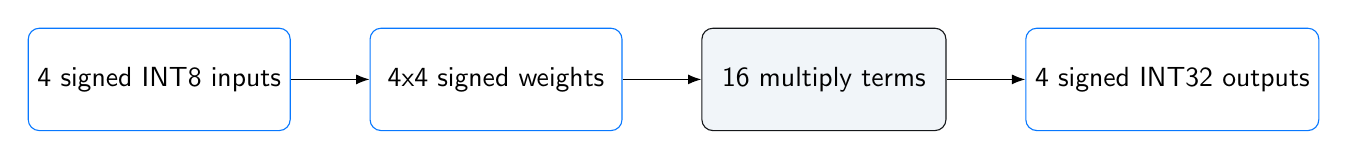
\begin{tikzpicture}[node distance=10mm,>=Latex]
\node[draw=Blue,rounded corners,minimum width=29mm,minimum height=13mm] (x) {4 signed INT8 inputs};
\node[draw=Blue,rounded corners,right=of x,minimum width=32mm,minimum height=13mm] (m) {4x4 signed weights};
\node[draw=Ink,fill=Pale,rounded corners,right=of m,minimum width=31mm,minimum height=13mm] (mac) {16 multiply terms};
\node[draw=Blue,rounded corners,right=of mac,minimum width=30mm,minimum height=13mm] (y) {4 signed INT32 outputs};
\draw[->] (x)--(m); \draw[->] (m)--(mac); \draw[->] (mac)--(y);
\end{tikzpicture}
\end{center}

The largest four-term magnitude is 65,536, well inside signed INT32. The optimized 17/18-bit intermediate widths are therefore range-correct for the frozen 4x4 contract.

This is a proof point for a central AI-hardware primitive, not a claim about a complete layer, neural network, memory hierarchy, accelerator platform or deployment.

\sectionpage{3. The RTL transformation}{Narrower and balanced accumulation}

The baseline sign-extends every 16-bit product to 32 bits and then expresses four wide additions per output. The optimized version first adds product pairs at 17 bits, then combines the two pair sums at 18 bits and finally sign-extends the exact result.

\begin{tabularx}{\textwidth}{@{}X X@{}}
\toprule
\textbf{Frozen baseline} & \textbf{Optimized RTL}\\
\midrule
16 products & 16 identical products\\
16 separate 32-bit extensions & No full-width product-extension bank\\
Four wide accumulation expressions & Balanced two-level adder trees\\
32-bit internal add operands & Range-correct 17/18-bit intermediates\\
\bottomrule
\end{tabularx}

\begin{lstlisting}
// Optimized structure for one output row
s00 = {p00[15], p00} + {p01[15], p01};
s01 = {p02[15], p02} + {p03[15], p03};
d0  = {s00[16], s00} + {s01[16], s01};
y0  = {{14{d0[17]}}, d0};
\end{lstlisting}

The exact public before/after patch is shipped with the case. No interface, protocol, arithmetic convention or output width is part of the optimization freedom.

\sectionpage{4. Correctness before PPA}{Fail closed verification}

The candidate reaches PPA scoring only after all earlier gates pass:

\begin{enumerate}[leftmargin=8mm]
\item SystemVerilog structure and synthesis safety.
\item \FunctionalTests\ deterministic golden simulations, including signed extremes, individual lanes, individual rows and seeded-random vectors.
\item Unbounded Yosys combinational equivalence of all four outputs for every possible 160-bit input assignment.
\item Width-sensitive synthesis and implementation checks that reject unsupported or oversized multiplier structures.
\item VTR route, timing and power extraction for every required pair.
\end{enumerate}

An inconclusive formal result, missing metric, timeout, route failure or functional mismatch is invalid. It cannot receive an improvement score.

\begin{tabularx}{\textwidth}{@{}lXr@{}}
\toprule
\textbf{Gate} & \textbf{Scope} & \textbf{Result}\\
\midrule
Golden simulation & 151 deterministic signed/extreme cases & \textcolor{Green}{\textbf{PASS}}\\
Formal equivalence & Every 160-bit input assignment & \textcolor{Green}{\textbf{PASS}}\\
PPA validity & Resource, multiplier-width and extraction limits & \textcolor{Green}{\textbf{PASS}}\\
Independent replay & Baseline and optimized paired records & \textcolor{Green}{\textbf{EXACT}}\\
\bottomrule
\end{tabularx}

\sectionpage{5. Measurement and certification}{Search evidence is not acceptance evidence}

The implementation target matches the academic VTR/PTM operating point used by the SHA-1 methodology case: a homogeneous LUT6 FPGA architecture, PTM 45 nm model, 0.9 V, 85 degrees C and a pinned Linux/amd64 toolchain image.

\begin{center}
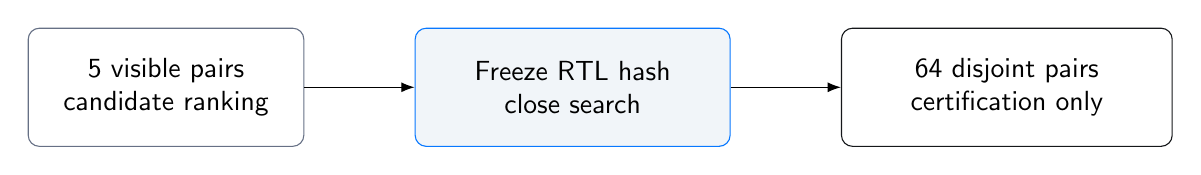
\begin{tikzpicture}[node distance=14mm,>=Latex]
\node[draw=Muted,rounded corners,align=center,minimum width=35mm,minimum height=15mm] (search) {\SearchPairs\ visible pairs\\candidate ranking};
\node[draw=Blue,fill=Pale,rounded corners,align=center,right=of search,minimum width=40mm,minimum height=15mm] (freeze) {Freeze RTL hash\\close search};
\node[draw=Ink,rounded corners,align=center,right=of freeze,minimum width=42mm,minimum height=15mm] (cert) {\CertificationPairs\ disjoint pairs\\certification only};
\draw[->] (search)--(freeze); \draw[->] (freeze)--(cert);
\end{tikzpicture}
\end{center}

The score is the paired geometric mean of total area, critical-path delay and active-total-power ratios. Lower is better. Acceptance is fixed before measurement: the composite one-sided 95\% upper confidence bound must be below 1.0, while no primary metric may have a one-sided 95\% lower bound above 1.0.

The public compact certificate retains all \CertificationPairs\ baseline/optimized metric pairs under blinded pair labels. It does not publish the optimization implementation, private execution data or reserved placement identities.

\sectionpage{6. Certified result}{Paired estimates over the fixed held-out sample}

\begin{tabularx}{\textwidth}{@{}lYYY@{}}
\toprule
\textbf{Metric} & \textbf{Estimate} & \textbf{Two-sided 95\% interval} & \textbf{Wins / losses}\\
\midrule
Area improvement & \AreaImprovement\% & \AreaLow\% to \AreaHigh\% & \AreaWins\ / \AreaLosses\\
Delay improvement & \DelayImprovement\% & \DelayLow\% to \DelayHigh\% & \DelayWins\ / \DelayLosses\\
Active-power improvement & \PowerImprovement\% & \PowerLow\% to \PowerHigh\% & \PowerWins\ / \PowerLosses\\
Composite improvement & \CompositeImprovement\% & \CompositeLow\% to \CompositeHigh\% & \CompositeWins\ / \CompositeLosses\\
\bottomrule
\end{tabularx}

Area and active power improve in all 64 pairs. Critical-path delay improves in 54 and regresses in 10, while its paired estimate and non-regression bound still pass. The composite improves in every held-out pair.

\begin{claimbox}
\textbf{Interpretation.} The composite estimate is a target-specific modeled comparison. It supports a reproducible result on the frozen academic architecture, not a universal 8.3230\% improvement for every device, toolchain or workload.
\end{claimbox}

\sectionpage{7. Public trust boundary}{What a client can inspect}

The public case includes the baseline and optimized RTL, exact patch, compact paired certificate, checksums, this report and a fail-closed Python verifier. From the case directory:

\begin{lstlisting}
python3 verify.py
\end{lstlisting}

The verifier checks file identities, the exact RTL patch, schema strictness, all paired values, derived area/power/frequency relationships, geometric aggregates, confidence intervals, acceptance bounds, resource limits and independent-replay attestations.

\begin{tabularx}{\textwidth}{@{}X X@{}}
\toprule
\textbf{Public evidence} & \textbf{Outside the public package}\\
\midrule
Before/after RTL and patch & Optimization implementation\\
Paired compact measurements & Private execution data\\
Correctness and replay attestations & Internal search history\\
Tool and target identities & Future reserved certification pools\\
\bottomrule
\end{tabularx}

\textbf{Baseline RTL SHA-256}\\[-1mm]
\hash{\BaselineHash}\\[3mm]
\textbf{Optimized RTL SHA-256}\\[-1mm]
\hash{\OptimizedHash}\\[3mm]
\textbf{Compact certificate SHA-256}\\[-1mm]
\hash{\CertificateHash}

\vfill
\begin{claimbox}
\textbf{Commercial next step.} A customer pilot should freeze one owned design interface, define success and validity limits before search, select an implementation target and agree which evidence may be published. Results remain subject to that target and contract.
\end{claimbox}

\end{document}
